% !TeX program = xelatex
\documentclass[a4paper,10pt]{article}

% ============================================================================
% ១. កញ្ចប់បណ្ណាល័យ និងការកំណត់ទំព័រ (Packages & Page Setup — តាមគំរូ ls_plan.tex)
% ============================================================================
\usepackage[a4paper, left=0.95cm, right=0.95cm, top=0.85cm, bottom=0.92cm, footskip=0.52cm]{geometry}
\usepackage{amsmath}
\usepackage{unicode-math}
\usepackage{fontspec}
\usepackage{longtable, array, multirow, colortbl}
\usepackage[table]{xcolor}
\usepackage{enumitem}
\usepackage{pifont}
\usepackage{fancyhdr}
\usepackage{tikz}
\usetikzlibrary{calc, arrows.meta, decorations.pathreplacing, patterns, positioning, babel}

\makeatletter
\let\@expl@@@mark@update@singlecol@structures@@\relax
\makeatother

% --- ប្រព័ន្ធស្វែងរកទីតាំងពុម្ពអក្សរស្វ័យប្រវត្តិ (Windows Local + Cloud Repo fonts/) ---
\providecommand{\NGSFindFonts}{%
  \IfFileExists{C:/Windows/Fonts/cambria.ttc}{%
    \def\NGSSysPath{C:/Windows/Fonts/}%
    \def\NGSUserPath{C:/Users/KIT/AppData/Local/Microsoft/Windows/Fonts/}%
  }{%
    \IfFileExists{./fonts/KhmerOSsiemreap.ttf}{\def\NGSSysPath{./fonts/}\def\NGSUserPath{./fonts/}}{%
    \IfFileExists{../fonts/KhmerOSsiemreap.ttf}{\def\NGSSysPath{../fonts/}\def\NGSUserPath{../fonts/}}{%
    \IfFileExists{../../fonts/KhmerOSsiemreap.ttf}{\def\NGSSysPath{../../fonts/}\def\NGSUserPath{../../fonts/}}{%
    \IfFileExists{../../../fonts/KhmerOSsiemreap.ttf}{\def\NGSSysPath{../../../fonts/}\def\NGSUserPath{../../../fonts/}}{%
    \IfFileExists{../../../../fonts/KhmerOSsiemreap.ttf}{\def\NGSSysPath{../../../../fonts/}\def\NGSUserPath{../../../../fonts/}}{%
    \IfFileExists{../../../../../fonts/KhmerOSsiemreap.ttf}{\def\NGSSysPath{../../../../../fonts/}\def\NGSUserPath{../../../../../fonts/}}{%
    \IfFileExists{../../../../../../fonts/KhmerOSsiemreap.ttf}{\def\NGSSysPath{../../../../../../fonts/}\def\NGSUserPath{../../../../../../fonts/}}{%
      \def\NGSSysPath{../../../../../../../fonts/}\def\NGSUserPath{../../../../../../../fonts/}%
    }}}}}}}%
  }%
}
\NGSFindFonts

% ============================================================================
% ២. កំណត់ពុម្ពអក្សរ (Fonts — តាមគំរូ ls_plan.tex)
% ============================================================================
\setmathfont[Path={\NGSSysPath}, FontIndex=1, Scale=1.02]{cambria.ttc}
\defaultfontfeatures{Ligatures=TeX}

\setmainfont[
  Path={\NGSUserPath},
  Extension=.ttf,
  Script=Khmer,
  BoldFont={KhmerOSsiemreap},
  BoldFeatures={FakeBold=1.8},
  ItalicFont={KhmerOSsiemreap},
  ItalicFeatures={FakeSlant=0.25},
  BoldItalicFont={KhmerOSsiemreap},
  BoldItalicFeatures={FakeBold=1.8, FakeSlant=0.25}
]{KhmerOSsiemreap}

\newfontfamily\muol[Path={\NGSUserPath}, Extension=.ttf, Script=Khmer]{KhmerOSmuollight}
\newfontfamily\Tacteing[Path={\NGSUserPath}, Extension=.TTF]{TACTENG}
\newfontfamily\TimesEn[Path={\NGSSysPath}, Extension=.ttf, BoldFont={timesbd}, ItalicFont={timesi}, BoldItalicFont={timesbi}]{times}
\newfontfamily\CalibriFont[Path={\NGSSysPath}, Extension=.ttf]{calibri}
\newfontfamily\CourierCirc[Path={\NGSSysPath}, Extension=.ttf]{cour}

\XeTeXlinebreaklocale "km"
\XeTeXlinebreakskip = 0pt plus 1pt minus 0.1pt

% ============================================================================
% ៣. ពណ៌ និងការតុបតែង (Colors & Styles)
% ============================================================================
\definecolor{stepbg}{HTML}{D9D9D9}
\definecolor{headgray}{HTML}{E6E6E6}
\definecolor{emphred}{HTML}{C00000}

\pagestyle{fancy}
\fancyhf{}
\renewcommand{\headrulewidth}{0pt}
\fancyfoot[R]{\CalibriFont\fontsize{9pt}{11pt}\selectfont\thepage}

\setlength{\parindent}{0pt}
\setlength{\parskip}{0pt}
\setlength{\tabcolsep}{4.5pt}
\setlength{\LTpre}{2pt}
\setlength{\LTpost}{2pt}

\newcolumntype{L}[1]{>{\raggedright\arraybackslash}p{#1}}
\newcolumntype{C}[1]{>{\centering\arraybackslash}p{#1}}

% ============================================================================
% ៤. ពាក្យបញ្ជាជំនួយ (Helper Macros)
% ============================================================================
\newcommand{\en}[1]{{\TimesEn #1}}
\newcommand{\enbf}[1]{{\TimesEn\bfseries #1}}
\newcommand{\khmflourish}{{\Tacteing\fontsize{15pt}{15pt}\selectfont 3}}
\newcommand{\wcirc}{{\CourierCirc\fontsize{9.5pt}{11pt}\selectfont o}}
\newcommand{\ditem}{{\fontsize{7.5pt}{10pt}\selectfont\ding{117}}\ }
\newcommand{\fiveE}[1]{\textcolor{emphred}{\CalibriFont\bfseries #1}}
\newcommand{\redsub}[1]{\textcolor{emphred}{#1}}
\newcommand{\timenote}[1]{\textcolor{emphred}{\textit{#1}}}
\newcommand{\stepheader}[1]{\multicolumn{3}{|c|}{\cellcolor{stepbg}\muol #1} \\ \hline}
\newcommand{\cfig}[1]{{\centering\vspace{3pt}#1\vspace{3pt}\par}}
\newcommand{\cnum}[1]{\mbox{\fontsize{10.5pt}{12pt}\selectfont\ding{\numexpr181+#1\relax}}}
\newcommand{\unit}[1]{\,\text{\en{#1}}}
\newcommand{\riel}{\,\text{៛}}
\newcommand{\graybox}[1]{\colorbox{headgray}{\strut #1}}

% ============================================================================
% ៥. រូបភាព TikZ ស-ខ្មៅ សម្រាប់បង្រៀនលើក្ដារខៀន និងសន្លឹកកិច្ចការ (B&W Diagrams)
% ============================================================================

% ១. E1 Engage: អន្ទាក់ឈប់មុនអស់លទ្ធភាពក្នុង A = x^3 - 2x^2 - 4x + 8 (ទំ.៧១--៧២)
\newcommand{\figEngageALGFiveEight}{%
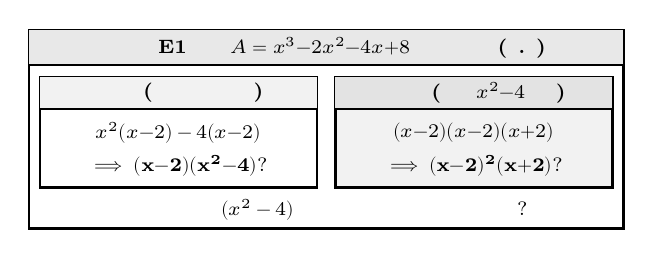
\begin{tikzpicture}[x=1cm, y=1cm, every node/.style={font=\scriptsize, text=black}]
  \draw[black, line width=0.9pt] (0,0) rectangle (7.55,2.52);
  \fill[gray!18] (0,2.08) rectangle (7.55,2.52);
  \draw[black, line width=0.6pt] (0,2.08) -- (7.55,2.08);
  \node at (3.775,2.30) {\textbf{បេសកកម្ម \en{E1}៖ ដាក់ $A = x^3{-}2x^2{-}4x{+}8$ ឱ្យអស់លទ្ធភាព (ទំ.៧១)}};

  % Student A
  \draw[black, line width=0.8pt] (0.14,0.52) rectangle (3.66,1.92);
  \fill[gray!10] (0.14,1.52) rectangle (3.66,1.92);
  \draw[black, line width=0.5pt] (0.14,1.52) -- (3.66,1.52);
  \node at (1.90,1.72) {\textbf{សិស្ស ក (ឈប់ត្រឹមដឺក្រេទី ២)}};
  \node at (1.90,1.22) {$x^2(x{-}2) - 4(x{-}2)$};
  \node at (1.90,0.80) {$\implies \mathbf{(x{-}2)(x^2{-}4)}$?};

  % Student B
  \draw[black, line width=0.95pt, fill=gray!10] (3.89,0.52) rectangle (7.41,1.92);
  \fill[gray!22] (3.89,1.52) rectangle (7.41,1.92);
  \draw[black, line width=0.55pt] (3.89,1.52) -- (7.41,1.52);
  \node at (5.65,1.72) {\textbf{សិស្ស ខ (បំបែក $x^2{-}4$ បន្ត)}};
  \node at (5.65,1.22) {$(x{-}2)(x{-}2)(x{+}2)$};
  \node at (5.65,0.80) {$\implies \mathbf{(x{-}2)^2(x{+}2)}$?};

  \node at (3.775,0.24) {\textbf{ពិនិត្យ៖} តើកត្តា $(x^2 - 4)$ អាចបំបែកជាកត្តាដឺក្រេទី ១ បន្តទៀតបានឬទេ?};
\end{tikzpicture}}

% ២. E2 Explore: បំពេញការេទ្វេធា និងបំបែកតួកណ្ដាល (ទំ.៧១)
\newcommand{\figExploreALGFiveEight}{%
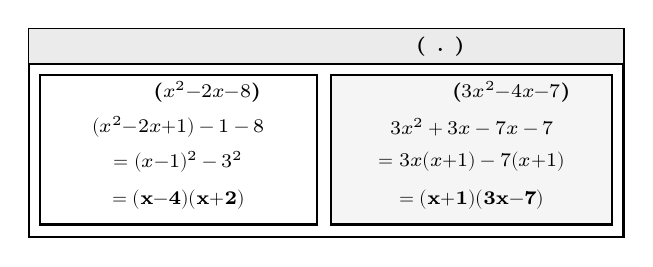
\begin{tikzpicture}[x=1cm, y=1cm, every node/.style={font=\scriptsize, text=black}]
  \draw[black, line width=0.9pt] (0,0) rectangle (7.55,2.64);
  \fill[gray!16] (0,2.20) rectangle (7.55,2.64);
  \draw[black, line width=0.6pt] (0,2.20) -- (7.55,2.20);
  \node at (3.775,2.42) {\textbf{វិធីបំពេញការេទ្វេធា និងវិធីបំបែកតួកណ្ដាល (ទំ.៧១)}};

  % Left: Completing the square
  \draw[black, line width=0.8pt] (0.14,0.16) rectangle (3.66,2.06);
  \node at (1.90,1.84) {\textbf{បំពេញការេ ($x^2{-}2x{-}8$)}};
  \node at (1.90,1.40) {$(x^2{-}2x{+}1) - 1 - 8$};
  \node at (1.90,0.96) {$= (x{-}1)^2 - 3^2$};
  \node at (1.90,0.48) {$= \mathbf{(x{-}4)(x{+}2)}$};

  % Right: Splitting middle term
  \draw[black, line width=0.8pt, fill=gray!8] (3.84,0.16) rectangle (7.41,2.06);
  \node at (5.625,1.84) {\textbf{បំបែកតួកណ្ដាល ($3x^2{-}4x{-}7$)}};
  \node at (5.625,1.40) {$3x^2 + 3x - 7x - 7$};
  \node at (5.625,0.96) {$= 3x(x{+}1) - 7(x{+}1)$};
  \node at (5.625,0.48) {$= \mathbf{(x{+}1)(3x{-}7)}$};
\end{tikzpicture}}

% ៣. E3 Explain: សង្ខេបយុទ្ធវិធីទាំង ៣ ក្នុងចំណុច ៤.៣ (ទំ.៧១--៧២)
\newcommand{\figRuleALGFiveEight}{%
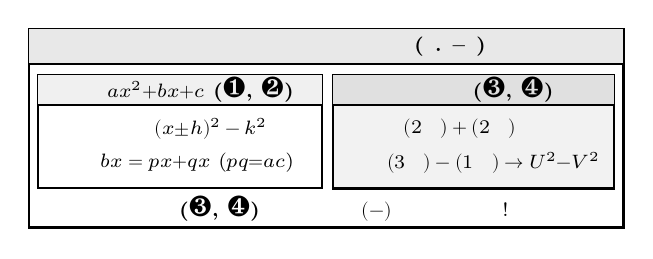
\begin{tikzpicture}[x=1cm, y=1cm, every node/.style={font=\scriptsize, text=black}]
  \draw[black, line width=0.9pt] (0,0) rectangle (7.55,2.52);
  \fill[gray!18] (0,2.08) rectangle (7.55,2.52);
  \draw[black, line width=0.6pt] (0,2.08) -- (7.55,2.08);
  \node at (3.775,2.30) {\textbf{យុទ្ធវិធីទាំង ៣ នៃការដាក់កន្សោមជាផលគុណកត្តា (ទំ.៧១--៧២)}};

  % Left: Trinomial strategies
  \draw[black, line width=0.8pt] (0.12,0.50) rectangle (3.72,1.94);
  \fill[gray!12] (0.12,1.56) rectangle (3.72,1.94);
  \draw[black, line width=0.55pt] (0.12,1.56) -- (3.72,1.56);
  \node at (1.92,1.75) {\textbf{ត្រីធា $ax^2{+}bx{+}c$ (\cnum{1}, \cnum{2})}};
  \node at (1.92,1.26) {បំពេញការេ៖ $(x{\pm}h)^2 - k^2$};
  \node at (1.92,0.82) {បំបែក $bx = px{+}qx$ ($pq{=}ac$)};

  % Right: Grouping 4 terms
  \draw[black, line width=0.95pt, fill=gray!10] (3.86,0.50) rectangle (7.43,1.94);
  \fill[gray!24] (3.86,1.56) rectangle (7.43,1.94);
  \draw[black, line width=0.6pt] (3.86,1.56) -- (7.43,1.56);
  \node at (5.645,1.75) {\textbf{ផ្ដុំតួ ៤ តួ (\cnum{3}, \cnum{4})}};
  \node at (5.645,1.26) {ផ្ដុំ $(2\text{ តួ}) + (2\text{ តួ})$ រកកត្តារួម};
  \node at (5.645,0.82) {ឬផ្ដុំ $(3\text{ តួ}) - (1\text{ តួ}) \to U^2{-}V^2$};

  \node at (3.775,0.24) {\textbf{ចំណាំ (\cnum{3}, \cnum{4})៖} ប្ដូរសញ្ញាក្រោយ $(-)$ និងបំបែកកត្តាឱ្យអស់!};
\end{tikzpicture}}

% ៤. E4 Elaborate: ផ្ដុំ ៣ តួដក ១ តួ និងគូបរួម (ទំ.៧១--៧២, ៧៤)
\newcommand{\figElaborateALGFiveEight}{%
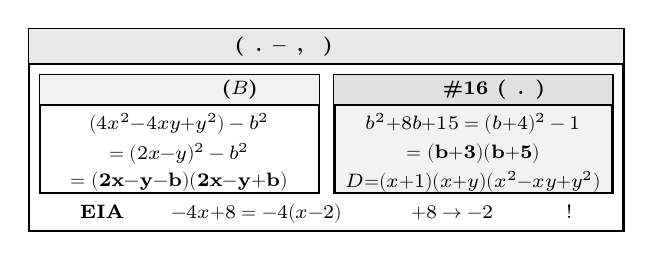
\begin{tikzpicture}[x=1cm, y=1cm, every node/.style={font=\scriptsize, text=black}]
  \draw[black, line width=0.9pt] (0,0) rectangle (7.55,2.56);
  \fill[gray!18] (0,2.12) rectangle (7.55,2.56);
  \draw[black, line width=0.6pt] (0,2.12) -- (7.55,2.12);
  \node at (3.775,2.34) {\textbf{លំហាត់គំរូ (ទំ.៧១--៧២, ៧៤)៖ ផ្ដុំ ៣ តួ និងបំពេញការេ}};

  % Left
  \draw[black, line width=0.8pt] (0.14,0.48) rectangle (3.68,1.98);
  \fill[gray!12] (0.14,1.60) rectangle (3.68,1.98);
  \draw[black, line width=0.55pt] (0.14,1.60) -- (3.68,1.60);
  \node at (1.91,1.79) {\textbf{ផ្ដុំ ៣ តួ ដក ១ តួ ($B$)}};
  \node at (1.91,1.36) {$(4x^2{-}4xy{+}y^2) - b^2$};
  \node at (1.91,0.98) {$= (2x{-}y)^2 - b^2$};
  \node at (1.91,0.62) {$= \mathbf{(2x{-}y{-}b)(2x{-}y{+}b)}$};

  % Right
  \draw[black, line width=0.95pt, fill=gray!10] (3.88,0.48) rectangle (7.41,1.98);
  \fill[gray!24] (3.88,1.60) rectangle (7.41,1.98);
  \draw[black, line width=0.6pt] (3.88,1.60) -- (7.41,1.60);
  \node at (5.645,1.79) {\textbf{លំហាត់ \en{\#16} (ទំ.៧៤)}};
  \node at (5.645,1.36) {$b^2{+}8b{+}15 = (b{+}4)^2 - 1$};
  \node at (5.645,0.98) {$= \mathbf{(b{+}3)(b{+}5)}$};
  \node at (5.645,0.62) {$D{=}(x{+}1)(x{+}y)(x^2{-}xy{+}y^2)$};

  \node at (3.775,0.22) {\textbf{\en{EIA}៖} ក្នុង $-4x{+}8 = -4(x{-}2)$ ត្រូវប្ដូរ $+8 \to -2$ ក្រោយសញ្ញាដក!};
\end{tikzpicture}}

% ៥. E5 Evaluate: ជម្រើសវិនិច្ឆ័យ A-D ដាក់ x^2 - 5x + 6 ជាផលគុណកត្តា
\newcommand{\figExitALGFiveEight}{%
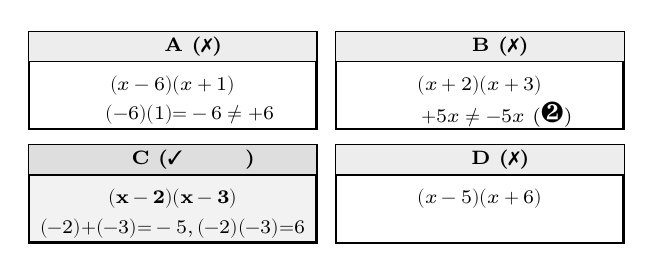
\begin{tikzpicture}[x=1cm, y=1cm, every node/.style={font=\scriptsize, text=black}]
  % Choice A
  \draw[black, line width=0.8pt] (0,1.44) rectangle (3.65,2.68);
  \fill[gray!14] (0,2.30) rectangle (3.65,2.68);
  \draw[black, line width=0.5pt] (0,2.30) -- (3.65,2.30);
  \node at (1.825,2.49) {\textbf{ជម្រើស \en{A} (\ding{55})}};
  \node at (1.825,2.00) {$(x - 6)(x + 1)$};
  \node at (1.825,1.62) {ផលគុណ $(-6)(1){=}-6 \neq +6$};

  % Choice B
  \draw[black, line width=0.8pt] (3.90,1.44) rectangle (7.55,2.68);
  \fill[gray!14] (3.90,2.30) rectangle (7.55,2.68);
  \draw[black, line width=0.5pt] (3.90,2.30) -- (7.55,2.30);
  \node at (5.725,2.49) {\textbf{ជម្រើស \en{B} (\ding{55})}};
  \node at (5.725,2.00) {$(x + 2)(x + 3)$};
  \node at (5.725,1.62) {ផលបូក $+5x \neq -5x$ (\cnum{2})};

  % Choice C (Correct)
  \draw[black, line width=1.0pt, fill=gray!10] (0,0) rectangle (3.65,1.24);
  \fill[gray!26] (0,0.86) rectangle (3.65,1.24);
  \draw[black, line width=0.55pt] (0,0.86) -- (3.65,0.86);
  \node at (1.825,1.05) {\textbf{ជម្រើស \en{C} (\ding{51} ត្រឹមត្រូវ)}};
  \node at (1.825,0.56) {$\mathbf{(x - 2)(x - 3)}$};
  \node at (1.825,0.18) {$(-2){+}(-3){=}-5, (-2)(-3){=}6$};

  % Choice D
  \draw[black, line width=0.8pt] (3.90,0) rectangle (7.55,1.24);
  \fill[gray!14] (3.90,0.86) rectangle (7.55,1.24);
  \draw[black, line width=0.5pt] (3.90,0.86) -- (7.55,0.86);
  \node at (5.725,1.05) {\textbf{ជម្រើស \en{D} (\ding{55})}};
  \node at (5.725,0.56) {$(x - 5)(x + 6)$};
  \node at (5.725,0.18) {យកមេគុណដាក់ត្រង់ៗខុសក្បួន};
\end{tikzpicture}}

% ============================================================================
% ៦. ចាប់ផ្ដើមឯកសារ (Document Body)
% ============================================================================
\begin{document}
\fontsize{10pt}{15.2pt}\selectfont

% --- ក្បាលរដ្ឋបាល (Administrative Header) ---
\begin{center}
  {\muol\fontsize{11pt}{16pt}\selectfont ព្រះរាជាណាចក្រកម្ពុជា}\\[2pt]
  {\muol\fontsize{11pt}{16pt}\selectfont ជាតិ សាសនា ព្រះមហាក្សត្រ}\\[-2pt]
  \khmflourish
\end{center}
\vspace{-4pt}

{\muol\fontsize{10pt}{15pt}\selectfont
មន្ទីរអប់រំ យុវជន និងកីឡា ខេត្តកំពង់ធំ\\
ការិយាល័យអប់រំ យុវជន និងកីឡា ស្រុកកំពង់ស្វាយ\\
អនុវិទ្យាល័យព្រះក្រសាំង}

\vspace{2pt}
\begin{center}
  {\muol\fontsize{12pt}{18pt}\selectfont កិច្ចតែងការបង្រៀន}
\end{center}
\vspace{1pt}

% --- ព័ត៌មានទូទៅ (General Metadata) ---
\begin{tabular}{@{}p{1.85cm}p{3.25cm}@{\hspace{4pt}:\hspace{6pt}}p{12.65cm}@{}}
  & - \quad មុខវិជ្ជា          & គណិតវិទ្យា ថ្នាក់ទី៨ (ពីជគណិត) \\
  & - \quad ចំណងជើងមេរៀន & មេរៀនទី៥៖ កន្សោមពីជគណិត \\
  & - \quad ចំណងជើងរង      & ៤.៣ របៀបផ្សេងៗក្នុងការដាក់កន្សោមជាផលគុណកត្តា \\
  & - \quad រយៈពេល             & ១ ម៉ោងសិក្សា (៥០ នាទី) \\
  & - \quad បង្រៀនដោយ         & ហុក ប៊ុនថែន \\
  & - \quad កាលបរិច្ឆេទ        & ថ្ងៃសៅរ៍ ទី១២ ខែធ្នូ ឆ្នាំ២០២៦ \\
\end{tabular}

\vspace{4pt}

% --- I. វត្ថុបំណង ---
{\muol\enbf{I.} វត្ថុបំណង}\par\vspace{2pt}
\begin{tabular}{@{}p{0.55cm}p{2.55cm}@{\hspace{2pt}:\hspace{6pt}}L{15.4cm}@{}}
  & \wcirc វិជ្ជាសម្បទា   & សិស្សប្រាប់បាននូវវិធីទាំង ៣ ក្នុងការដាក់កន្សោមជាផលគុណកត្តា គឺការបំពេញការេទ្វេធា ការបំបែកតួកណ្ដាល និងការផ្ដុំតួ (ទំ.៧១–៧២) ។ \\[2pt]
  & \wcirc បំណិនសម្បទា & សិស្សដាក់ត្រីធាដឺក្រេទី ២ និងពហុធា ៤ តួជាផលគុណកត្តាឱ្យអស់លទ្ធភាពលើសន្លឹកកិច្ចការបានត្រឹមត្រូវ ។ \\[2pt]
  & \wcirc ចរិយាសម្បទា  & សិស្សមានទម្លាប់ពិនិត្យសញ្ញាក្នុងវង់ក្រចកពេលផ្ដុំតួ និងបំបែកកត្តាបន្តរហូតអស់លទ្ធភាពប្រកបដោយភាពអត់ធ្មត់ ។ \\
\end{tabular}

\vspace{3pt}

% --- II. សម្ភារៈឧបទេស (Zero-LCD & Fill-In Worksheet Context) ---
{\muol\enbf{II.} សម្ភារៈឧបទេស}\par\vspace{2pt}
\hspace*{0.55cm}$\bullet$ សៀវភៅសិក្សាគោលថ្នាក់ទី៨ (ទំ.៧១--៧២, ៧៤) ក្ដារខៀន ដីស/ហ្វឺត បន្ទាត់ត្រង់ និង\textbf{សន្លឹកកិច្ចការសិស្សបំពេញចន្លោះ ស-ខ្មៅ} (កូដ \en{ALG58} ទំព័រ ១--២ សម្រាប់សិស្ស និងទំព័រ ៣ ប្លង់ក្ដារខៀន/ចម្លើយគ្រូ — គ្មានប្រើ \en{LCD})

\vspace{3pt}

% --- III. វិធីសាស្រ្តបង្រៀន ---
{\muol\enbf{III.} វិធីសាស្រ្តបង្រៀន}\par\vspace{2pt}
\begin{tabular}{@{}p{0.55cm}p{2.55cm}@{\hspace{2pt}:\hspace{6pt}}L{15.4cm}@{}}
  & $\bullet$ គោលវិធី      & សិស្សមជ្ឈមណ្ឌល (សន្លឹកកិច្ចការបំពេញចន្លោះជាគោល + ការពិភាក្សាជាក្រុមតូច ៣ នាក់) \\
  & $\bullet$ យុទ្ធវិធីបង្រៀន & គំរូស្ថាបនានិយម \en{5Es} រួមបញ្ចូល \textit{ភាពបត់បែននៃយុទ្ធវិធី (\en{Procedural Flexibility})} និង \textit{ការត្រួតពិនិត្យកត្តាអស់លទ្ធភាព} \\
\end{tabular}

\vspace{4pt}

% --- IV. ដំណើរការបង្រៀន (50-Minute 5E Flow) ---
{\muol\enbf{IV.} ដំណើរការបង្រៀន}\par\vspace{1pt}

\renewcommand{\arraystretch}{1.15}
\begin{longtable}{|L{5.50cm}|L{7.90cm}|L{4.80cm}|}
\hline
\multicolumn{1}{|c|}{\cellcolor{headgray}\muol សកម្មភាពគ្រូ} &
\multicolumn{1}{c|}{\cellcolor{headgray}\muol ខ្លឹមសារមេរៀន} &
\multicolumn{1}{c|}{\cellcolor{headgray}\muol សកម្មភាពសិស្ស} \\[2pt]
\hline
\endfirsthead

\hline
\multicolumn{1}{|c|}{\cellcolor{headgray}\muol សកម្មភាពគ្រូ} &
\multicolumn{1}{c|}{\cellcolor{headgray}\muol ខ្លឹមសារមេរៀន} &
\multicolumn{1}{c|}{\cellcolor{headgray}\muol សកម្មភាពសិស្ស} \\[2pt]
\hline
\endhead

\hline
\endfoot

% ==================== ជំហានទី១ (2min) ====================
\stepheader{ជំហានទី១ \enbf{(}រដ្ឋបាលថ្នាក់\enbf{)}}
$\bullet$ ពិនិត្យវត្តមាន អនាម័យ និងសណ្ដាប់ធ្នាប់ថ្នាក់រៀន \par
$\bullet$ រៀបចំក្រុមតូច ៣ នាក់ និងចែក\textbf{សន្លឹកកិច្ចការសិស្ស} (\en{ALG58} ទំព័រ ១–២)
&
$\bullet$ រដ្ឋបាលថ្នាក់ អនាម័យ និងវិន័យសិក្សា \par
$\bullet$ ចែកសន្លឹកកិច្ចការម្នាក់ ១ សន្លឹក សម្រាប់បំពេញតាមដំណាក់កាល \en{E1--E5}
&
$\circ$ ប្រធានថ្នាក់រាយការណ៍វត្តមានសិស្ស \par
$\circ$ ទទួលសន្លឹកកិច្ចការ សរសេរឈ្មោះ និងអង្គុយតាមក្រុម ៣ នាក់ \\
\hline

% ==================== ជំហានទី២ (9min: កំណែ ≤3m + រំលឹក 3m + E1 3m) ====================
\stepheader{ជំហានទី២ \enbf{(}កិច្ចការផ្ទះ \enbf{+} ទំនាក់ទំនងមេរៀនថ្មី\enbf{)}}
\ditem \textbf{កំណែកិច្ចការផ្ទះ (\enbf{$\le$ 3 min})} \par
$\bullet$ ហៅសិស្ស ២ នាក់ឡើងកែលំហាត់ទំ.៧០, \en{\#11} ខ និងទំ.៧៤ \en{\#12} ក, \en{\#14} ង លើក្ដារខៀន
&
\hspace*{0.15cm}\redsub{កំណែកិច្ចការផ្ទះ (ទំ.៧០ និង ទំ.៧៣–៧៤)} \par
$\bullet$ \textbf{ទំ.៧០ (ខ) និង \en{\#11} ខ៖} $(y+5)^2$; \quad $(a-4)(3a-5)$ \par
$\bullet$ \textbf{ទំ.៧៤៖} \en{\#12} ក) $2(2x-3)(2x-1)$; \ \en{\#12} ខ) $(7a-1)(4a-3)$; \ \en{\#13} ង) $(5x-4y)(5x+4y)$; \ \en{\#14} ង) $c(a-x)^2$
&
$\circ$ ផ្ទៀងចម្លើយ និងកែតម្រូវចូលសៀវភៅកិច្ចការផ្ទះ \\[3pt]

\ditem \textbf{រំលឹកមេរៀនទាក់ទង (\enbf{3min})} \par
$\bullet$ សួរ៖ «តើត្រូវបន្ថែមចំនួនប៉ុន្មានលើ $x^2 - 2x$ ដើម្បីបានការេទ្វេធា $(x-1)^2$? ចុះ $(x-1)^2 - 3^2$ ស្មើផលគុណអ្វី?»
&
\hspace*{0.15cm}\redsub{រំលឹកការេទ្វេធា និងផលដកពីរការេ $U^2 - V^2$} \par
$\bullet$ បន្ថែម $1^2 = 1$៖ $x^2 - 2x + 1 = (x - 1)^2$ \par
$\bullet$ ផលដកពីរការេ៖ $(x - 1)^2 - 3^2 = (x - 1 - 3)(x - 1 + 3) = (x - 4)(x + 2)$
&
$\circ$ ឆ្លើយ៖ «បន្ថែម $1$ បាន $(x-1)^2$ និងស្មើ $(x-4)(x+2)$!» \\[3pt]

\fiveE{E1 - Engage (3min)} \timenote{(កុំទាន់ផ្តល់ចម្លើយ)} \par
\ditem \textbf{បេសកកម្មអន្ទាក់ឈប់មុនអស់លទ្ធភាព (សន្លឹកកិច្ចការ \en{E1})} \par
$\bullet$ ឱ្យសិស្សអានប្រអប់ \en{E1} ពិនិត្យការដាក់ $A = x^3 - 2x^2 - 4x + 8$ ជាផលគុណកត្តា រវាងសិស្ស ក និងសិស្ស ខ
&
\redsub{បេសកកម្ម \en{E1}៖ ដាក់ $A = x^3 - 2x^2 - 4x + 8$ ឱ្យអស់លទ្ធភាព (ទំ.៧១)} \par
$\bullet$ \textbf{សិស្ស ក} ផ្ដុំតួហើយឈប់ត្រឹម $(x - 2)(x^2 - 4)$! \par
$\bullet$ \textbf{សិស្ស ខ} បំបែកបន្តបាន $(x - 2)^2(x + 2)$! តើអ្នកណាដាក់អស់លទ្ធភាព?
&
$\circ$ ពិនិត្យកត្តា $(x^2-4)$ ពិភាក្សាជាគូ និងគូស \ding{51} ក្នុងប្រអប់ \en{E1} \\[3pt]

&
\cfig{\figEngageALGFiveEight}
& \\
\hline

% ==================== ជំហានទី៣ (17min: E2 11m + E3 6m) ====================
\stepheader{ជំហានទី៣ \enbf{(}ខ្លឹមសារមេរៀនថ្មី\enbf{)}}
\fiveE{E2 - Explore (11min)} \par
$\bullet$ សរសេរចំណងជើងរង \textbf{៤.៣ របៀបផ្សេងៗក្នុងការដាក់កន្សោមជាផលគុណកត្តា} លើក្ដារខៀន \par
\ditem \textbf{សកម្មភាព ១៖ បំពេញការេទ្វេធា និងបំបែកតួកណ្ដាល (ទំ.៧១, \enbf{6min}, \en{E2-A})} \par
$\bullet$ ឱ្យសិស្សបំពេញឧទាហរណ៍ទី ១ និងឧទាហរណ៍ទី ៣ (ទំ.៧១) លើ \en{E2-A}
&
៤.៣ របៀបផ្សេងៗក្នុងការដាក់ជាផលគុណកត្តា (ទំ.៧១) \par
$\bullet$ \textbf{ឧទាហរណ៍ទី ១ (បំពេញការេទ្វេធា)៖} $A = x^2 - 2x - 8 = (x^2 - 2x + 1) - 1 - 8 = (x-1)^2 - 3^2 = \mathbf{(x - 4)(x + 2)}$ \par
$\bullet$ \textbf{ឧទាហរណ៍ទី ៣ (បំបែកតួកណ្ដាល)៖} $F = 3x^2 - 4x - 7 = 3x^2 + 3x - 7x - 7 = 3x(x+1) - 7(x+1) = \mathbf{(x + 1)(3x - 7)}$
&
$\circ$ បំពេញជំហានបំពេញការេ និងបំបែកតួកណ្ដាលលើ \en{E2-A} \\[3pt]

\ditem \textbf{សកម្មភាព ២៖ បន្ថែម-ដកតួកណ្ដាល និងផ្ដុំតួ ៤ តួ (ទំ.៧១–៧២, \enbf{5min}, \en{E2-B})} \par
$\bullet$ ឱ្យសិស្សបំពេញឧទាហរណ៍ទី ២ និងលំហាត់គំរូ $A$ (ទំ.៧១–៧២) លើ \en{E2-B}
&
វិធីបន្ថែម-ដកតួកណ្ដាល និងផ្ដុំតួ ៤ តួ (ទំ.៧១–៧២) \par
$\bullet$ \textbf{ឧទាហរណ៍ទី ២៖} $E = 9t^4 - 28t^2 + 16 = (9t^4 - 24t^2 + 16) - 4t^2 = (3t^2 - 4)^2 - (2t)^2 = \mathbf{(3t^2 - 2t - 4)(3t^2 + 2t - 4)}$ \par
$\bullet$ \textbf{លំហាត់គំរូផ្ដុំតួ៖} $A = x^3 - 2x^2 - 4x + 8 = x^2(x-2) - 4(x-2) = (x-2)(x^2-4) = \mathbf{(x - 2)^2(x + 2)}$
&
$\circ$ ផ្ដុំតួ ចាប់កត្តារួម និងបំបែក $x^2-4$ បន្តលើ \en{E2-B} \\[3pt]

&
\cfig{\figExploreALGFiveEight}
& \\[3pt]

% --- E3 Explain (6min) ---
\fiveE{E3 - Explain (6min)} \par
$\bullet$ ដឹកនាំសិស្សសង្ខេបយុទ្ធវិធីទាំង ៣ ក្នុងការដាក់ជាផលគុណកត្តា (ទំ.៧១–៧២)
&
$\bullet$ \textbf{សង្ខេបយុទ្ធវិធីទាំង ៣ (ទំ.៧១–៧២)៖} \par
\hspace*{0.15cm}– \textbf{១) បំពេញការេទ្វេធា៖} បម្លែងជា $\graybox{$(x \pm h)^2 - k^2$}$ រួចប្រើ $U^2 - V^2$ \par
\hspace*{0.15cm}– \textbf{២) បំបែកតួកណ្ដាល ($ax^2+bx+c$)៖} បំបែក $bx = px + qx$ ដែល $\graybox{$p+q=b,\ pq=ac$}$ \par
\hspace*{0.15cm}– \textbf{៣) ផ្ដុំតួ ៤ តួ៖} ផ្ដុំជា $(2\text{ តួ}) + (2\text{ តួ})$ ឬ $(3\text{ តួ}) - (1\text{ តួ})$
&
$\circ$ បំពេញប្រអប់សង្ខេបយុទ្ធវិធីទាំង ៣ លើ \en{E3} \\[3pt]

$\bullet$ ភ្ជាប់\textbf{ធនាគារហេតុផល \cnum{1}--\cnum{4}} លើក្ដារខៀន និងសន្លឹកកិច្ចការ
&
\textbf{ធនាគារហេតុផល (\en{Warrant Bank})៖} \par
\cnum{1} \textbf{ថែមហើយត្រូវដកវិញ៖} បើបន្ថែម $+h^2$ ដើម្បីបំពេញការេទ្វេធា ត្រូវដក $-h^2$ មកវិញជានិច្ច \par
\cnum{2} \textbf{លក្ខខណ្ឌបំបែកតួកណ្ដាល៖} ពីរចំនួន $p, q$ ត្រូវផ្ទៀងទាំងផលបូក $p+q=b$ និងផលគុណ $pq=ac$
&
$\circ$ ផ្ទៀងលេខកូដ \cnum{1}--\cnum{2} លើសន្លឹកកិច្ចការ \\[3pt]

&
\cnum{3} \textbf{សញ្ញាក្រោយដកពេលផ្ដុំតួ៖} ពេលដាក់វង់ក្រចកក្រោយសញ្ញាដក $(-)$ ត្រូវប្ដូរសញ្ញាតួខាងក្នុង
&
$\circ$ ផ្ទៀងលេខកូដ \cnum{3} លើសន្លឹកកិច្ចការ \\[3pt]

&
\cnum{4} \textbf{បំបែកឱ្យអស់លទ្ធភាព៖} ត្រូវពិនិត្យកត្តាដឺក្រេទី ២ ឬទី ៣ ក្រែងអាចបំបែកបន្តទៀតបាន
&
$\circ$ ផ្ទៀងលេខកូដ \cnum{4} លើសន្លឹកកិច្ចការ \\[3pt]

&
\cfig{\figRuleALGFiveEight}
& \\
\hline

% ==================== ជំហានទី៤ (20min: E4 10m + E5 10m) ====================
\stepheader{ជំហានទី៤ \enbf{(}ពង្រីកចំណេះដឹង\enbf{)}}
\fiveE{E4 - Elaborate (10min)} \par
\ditem \textbf{លំហាត់គំរូ៖ ផ្ដុំតួ ៣ ទល់ ១ និងបំពេញការេ (ទំ.៧១–៧២, ៧៤)} \par
$\bullet$ ឱ្យសិស្សធ្វើលំហាត់គំរូ $B, C, D$ (ទំ.៧១–៧២) និងទំ.៧៤ \en{\#16} ក, ខ លើ \en{E4}
&
\textbf{លំហាត់គំរូពង្រីក (ទំ.៧១–៧២ និង ទំ.៧៤ \en{\#16})៖} \par
$\bullet$ \textbf{១) លំហាត់គំរូ $B, C, D$ (ទំ.៧១–៧២)៖} \par
\hspace*{0.15cm}-- $B = 4x^2 + y^2 - b^2 - 4xy = (2x-y)^2 - b^2 = \graybox{$(2x-y-b)(2x-y+b)$}$ \par
\hspace*{0.15cm}-- $C = (a-4)(y+2) - (a-4)(3y+2) = \mathbf{-2y(a - 4)}$ \par
\hspace*{0.15cm}-- $D = x^3(x+1) + y^3(x+1) = \mathbf{(x+1)(x+y)(x^2-xy+y^2)}$ \par
$\bullet$ \textbf{២) លំហាត់ \en{\#16} ក, ខ (ទំ.៧៤)៖} $A = b^2 + 8b + 15 = (b+4)^2 - 1 = \graybox{$(b+3)(b+5)$}$
&
$\circ$ ផ្ដុំតួ និងបំពេញការេលើ \en{E4} បានត្រឹមត្រូវ \\[3pt]

&
\cfig{\figElaborateALGFiveEight}
& \\[3pt]

$\bullet$ សួរសំណួរឆ្លុះបញ្ចាំង \textbf{\en{EIA Looking-Back}} (\enbf{1min})
&
\textbf{\en{EIA Looking-Back}៖} «ក្នុង $-4x + 8$ ហេតុអ្វីពេលចាប់ $-4$ ចេញ ក្នុងវង់ក្រចកក្លាយជា $(x - 2)$ មិនមែន $(x + 2)$?» ($\to$ ព្រោះ $(-4)(-2) = +8$ ប្ដូរសញ្ញាក្រោយដក \cnum{3}!)
&
$\circ$ ពន្យល់ដោយគុណបញ្ច្រាស $(-4)(x-2) = -4x+8$ \\[3pt]

% --- E5 Evaluate (10min) ---
\fiveE{E5 - Evaluate (10min)} \par
\ditem \textbf{ប្រតិបត្តិជាក្រុមតូច ៣ នាក់ (\enbf{4min}, សន្លឹកកិច្ចការ \en{E5})} \par
$\bullet$ ឱ្យសិស្សដោះស្រាយលំហាត់ទំ.៧៤ (\en{\#12} ច, \en{\#15} ក, ខ និង \en{\#16} គ)
&
\textbf{លំហាត់ប្រតិបត្តិ (ទំ.៧៤ \en{\#12, \#15, \#16})៖} \par
$\bullet$ \textbf{១) \en{\#12} ច និង \en{\#15} ក៖} $8ax - bx + 8ay - by = \mathbf{(8a - b)(x + y)}$; \quad $x^2 + 3x + 2 = \mathbf{(x + 1)(x + 2)}$ \par
$\bullet$ \textbf{២) \en{\#15} ខ និង \en{\#16} គ ($B$)៖} $3x^2 + 14x + 8 = \mathbf{(3x + 2)(x + 4)}$; \quad $x^2 + 4x + 3 = \mathbf{(x + 1)(x + 3)}$
&
$\circ$ ដាក់ជាផលគុណកត្តាជាក្រុមបានត្រឹមត្រូវទាំង ៤ លំហាត់ \\[3pt]

$\bullet$ ឱ្យក្រុមសិស្សផ្ទៀងផ្ទាត់និងបិទ\textbf{បេសកកម្ម \en{E1}} (\enbf{2min})
&
$\bullet$ \textbf{បិទបេសកកម្ម \en{E1}៖} សិស្ស ខ ត្រឹមត្រូវ! $x^3-2x^2-4x+8 = (x-2)(x^2-4) = \mathbf{(x-2)^2(x+2)}$ (\ding{51})!
&
$\circ$ បិទបេសកកម្ម \en{E1} ឃើញសិស្ស ខ ត្រឹមត្រូវ \\[3pt]

\ditem \textbf{សំណួរវិនិច្ឆ័យ \en{A--D} និងសំបុត្រចេញ (\enbf{4min})} \par
$\bullet$ ឱ្យសិស្សគូសរង្វង់ជម្រើសត្រូវលើសន្លឹកកិច្ចការ រួចលើកម្រាមដៃ ១--៤
&
\centering\textbf{សំណួរវិនិច្ឆ័យ \en{A--D}៖ ដាក់ត្រីធា $x^2 - 5x + 6$ ជាផលគុណកត្តា}\par
\textbf{\en{A.}} $(x - 6)(x + 1)$ \quad
\textbf{\en{B.}} $(x + 2)(x + 3)$ \quad
\textbf{\en{C.}} $(x - 2)(x - 3)$ \quad
\textbf{\en{D.}} $(x - 5)(x + 6)$\par
{\itshape (កត់សម្គាល់៖ រកពីរចំនួនដែលផលបូកស្មើ $-5$ និងផលគុណស្មើ $+6$)}
&
$\circ$ គណនា និងលើកម្រាមដៃ ៣ (\textbf{ជម្រើស \en{C}៖} $(x - 2)(x - 3)$) \\[3pt]

&
\cfig{\figExitALGFiveEight}
& \\[3pt]

$\bullet$ បញ្ជាក់ចម្លើយត្រូវ (\textbf{ជម្រើស \en{C}}) និងឱ្យបំពេញសំបុត្រចេញ ៦០ វិនាទី
&
$\bullet$ \textbf{សំបុត្រចេញ (ទំ.៧៤ \en{\#12} ឆ)៖} ដាក់ជាផលគុណកត្តា $ax + ay - 2bx - 2by = a(x+y) - 2b(x+y) = \mathbf{(x + y)(a - 2b)}$ ។
&
$\circ$ បំពេញសំបុត្រចេញលើសន្លឹកកិច្ចការមុនបញ្ចប់ម៉ោង \\
\hline

% ==================== ជំហានទី៥ (≤2min) ====================
\stepheader{ជំហានទី៥ \enbf{(}កិច្ចការផ្ទះ \enbf{+} បណ្ដាំផ្ញើ\enbf{)}}
\timenote{ចំណាយពេលឱ្យតិចបំផុតកុំឱ្យលើស 2min} \par
$\bullet$ ណែនាំប្រអប់កិច្ចការផ្ទះលើសន្លឹកកិច្ចការទំព័រ ២ (ទំ.៧៤ \en{\#12, \#15, \#16})
&
\centering\textbf{កិច្ចការផ្ទះ (សៀវភៅគោល ទំ.៧៤ លេខ ១២, ១៥, ១៦)}\par\raggedright
$\bullet$ \textbf{១) ទំ.៧៤ \en{\#12} ង និង \en{\#16} គ ($C$)៖} $(y - 8)(4y - 1) + y^2 - 8y$ និង $C = 4x^2 - 8x + 3$ ។ \par
$\bullet$ \textbf{២) ទំ.៧៤ \en{\#15} ឃ, ង, ជ៖} ដាក់ជាផលគុណកត្តា $2x^2 + 15x + 7$, $14a^2 + 18a - 20$ និង $6x^2 + 5x + 1$ ។
&
$\circ$ គូសចំណាំកិច្ចការផ្ទះលើសន្លឹកកិច្ចការ \\[3pt]

$\bullet$ ផ្តាំផ្ញើឱ្យរំលឹកមេរៀនទី៥ ទាំងមូល និងអានមុនមេរៀនទី៦ (កន្សោមសនិទាន)
&
$\bullet$ \textbf{បណ្ដាំផ្ញើ៖} រំលឹកវិធីដាក់កន្សោមជាផលគុណកត្តា និងអានមុន \textbf{មេរៀនទី៦៖ កន្សោមសនិទាន} (ទំ.៧៥–៧៦) ។
&
$\circ$ កត់ត្រាបណ្ដាំផ្ញើ ទុកសន្លឹកកិច្ចការក្នុងសៀវភៅ និងជម្រាបលាគ្រូ \\
\hline
\end{longtable}

\vspace{6pt}

% --- ហត្ថលេខា (Signature Block) ---
\begin{flushright}
  \begin{minipage}{8.6cm}
    \centering
    ថ្ងៃសៅរ៍ ៣កើត ខែមិគសិរ ឆ្នាំមមី អដ្ឋស័ក ពុទ្ធសករាជ ២៥៧០\\
    កំពង់ស្វាយ, ថ្ងៃទី១២ ខែធ្នូ ឆ្នាំ២០២៦\\[4pt]
    {\muol គ្រូបង្រៀន}\\[32pt]
    \hfill{\muol ហុក ប៊ុនថែន}\hspace*{1.4cm}
  \end{minipage}
\end{flushright}

\end{document}
